%%%%%%%%%%%%%%%%%%%%%%%%%%%%%%%%%%%%%%%%%%%%%%%%%
\chapter{Recursos Didáticos}
\section{Literatura Matemática}

\begin{enumerate}
\item O Teorema do Papagáio
\item O homem que calculava
\item Matemática divertida e curiosa
\item Matemática, cadê você?
\item Alex no país dos números
\item O diabo dos números
\item Incríveis passatempos matemáticos
\item Almanaque das curiosidades Matemáticas
\end{enumerate}
%http://www.esev.ipv.pt/mat1Ciclo/Nova%20pasta/_EM115_pp67-71_4f1d94c118b47_H.pdf
%http://www.sinprosp.org.br/congresso_matematica/revendo/dados/files/textos/Relatos/MATEM%C3%81TICA%20E%20LITERATURA%20INFANTIL_%20UMA%20NOVA%20E%20POSS%C3%8DVEL%20ABORDA.pdf
\section{Geogebra}
\section{Tablets e Smatphones}
\begin{multicols}{2}
Uma das diversas coisas que aprendi fazendo Matemática é que não há nada melhor que aprender enquanto se diverte. Conheci então alguns jogos que vem bem a calhar. Todos os jogos foram escolhidos do portal do \url{http://www.hypatiamat.com/jogosOnline.php}.
Todos os jogos do portal podem ser baixados via Google Play para a plataforma Android. Os que serão citados são aqueles que podem ser jogados através do computador online. Para o complemento de alguns jogos existe a possibilidade de efetuar login. Para isso basta se cadastrar no portal apartir de qualque jogo. Necessita apenas de um e-mail.

%\section{Jógos numéricos}

\subsection{Calculus}


\begin{center}
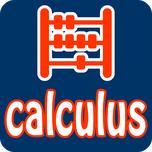
\includegraphics[scale=1]{./imagens/20.png}
\end{center}

Conteúdos abordados: Operações de soma, subtração e multiplicação nos números naturais.
Nesse jogo você pode escolher a dificuldade conforme a sua faixa etária. Nível de dificuldade é fácil.

\subsection{SAM}

\begin{center}
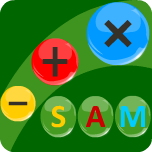
\includegraphics[scale=1]{./imagens/21.png}
\end{center}

Conteúdos abordados: Subtração, Adição e Multiplicação nos números naturais.

Efetuando login é possível verificar ranking. Online.


\subsection{SAMD}

\begin{center}
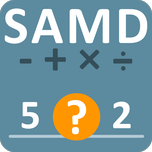
\includegraphics[scale=1]{./imagens/22.png}
\end{center}

Conteúdos abordados: Subtração, Adição, Multiplicação e Divisão nos números naturais e inteiros.

Efetuando login é possível verificar ranking. Online.

\subsection{Loto-SAMD}

\begin{center}
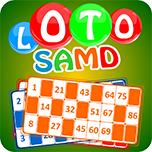
\includegraphics[scale=4]{./imagens/23.png}
\end{center}

Conteúdos abordados: Subtração, Adição, Multiplicação e Divisão nos números naturais.

Um jogo tipo logo em que as operações são chamadas e os resultados podem estar ou não no seu cartão. Caso esteja marque o valor com um feijão. Caso complete uma linha você ganha pontos estras. Ganha-se quando completa o cartão completo. São três tipos de cartão, um só com soma e subtração, o segundo é o anterior acrescido de multiplicação e o terceiro o anterior acrescido de divisão.

\subsection{SAMDuel}

\begin{center}
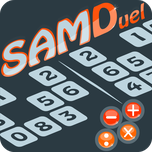
\includegraphics[scale=1]{./imagens/24.png}
\end{center}

Conteúdos abordados: Subtração, Adição, Multiplicação e Divisão nos números naturais e inteiros.

O resultado é dado e uma operação é definida. Nesse jogo você precisa escolher dois valores que compinados apartir da operação dada dê o resultado escolhido. Pode-se jogar contra a máquida ou contra um oponente.

\section{Jogos de estratégia}

\section{Jogos geométricos}

\section{Jogos de memória e puzzels}

\end{multicols}
